% ---
% Capa
% ---
\imprimircapa
% ---

% ---
% Folha de rosto
% (o * indica que haverá a ficha bibliográfica)
% ---
\imprimirfolhaderosto*
% ---

% ---
% Inserir a ficha bibliografica
% ---
% http://ficha.bu.ufsc.br/
\begin{fichacatalografica}
	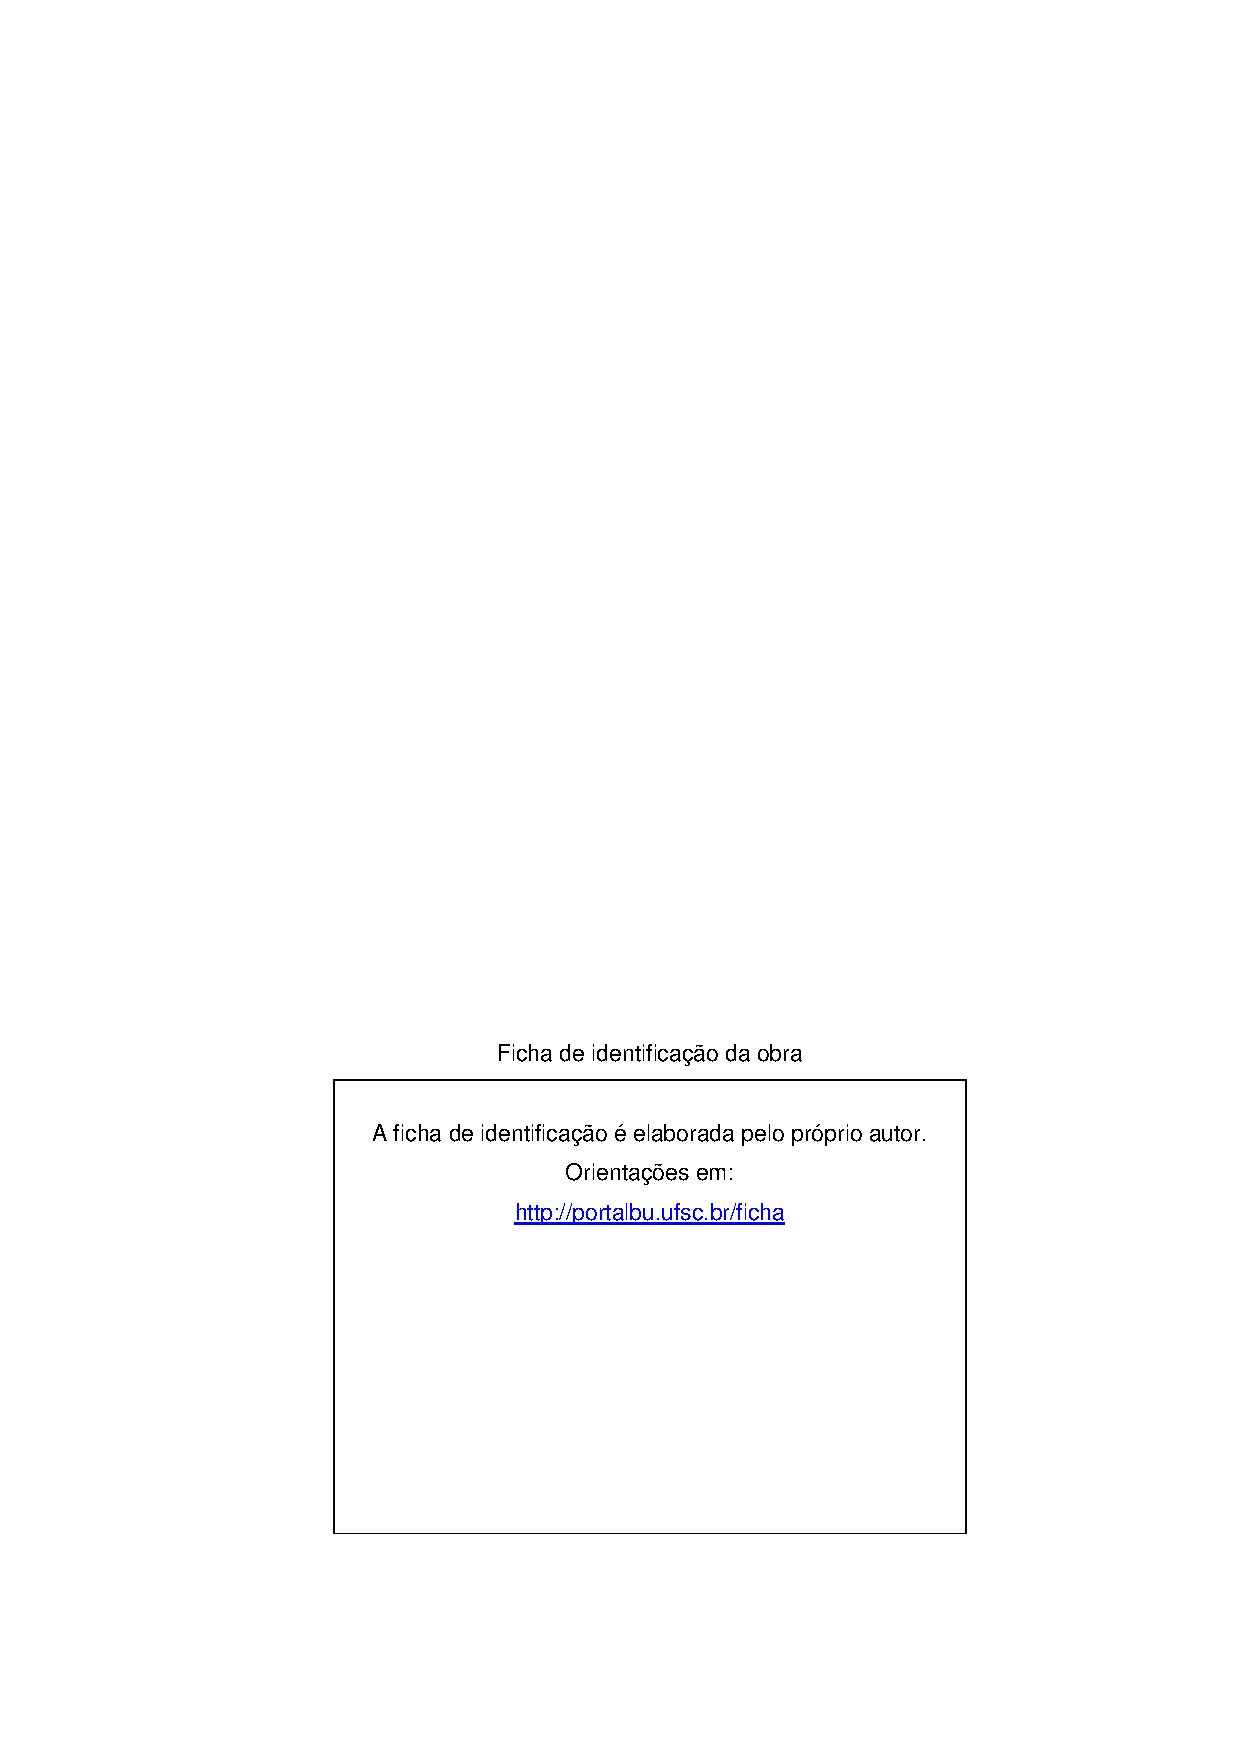
\includepdf{beforetext/Ficha_Catalografica.pdf}
\end{fichacatalografica}
% ---

% ---
% Inserir folha de aprovação
% ---
\begin{folhadeaprovacao}
	\OnehalfSpacing
	\centering
	\imprimirautor\\%
	\vspace*{10pt}		
	\textbf{\imprimirtitulo}%
	\ifnotempty{\imprimirsubtitulo}{:~\imprimirsubtitulo}\\%
	%		\vspace*{31.5pt}%3\baselineskip
	\vspace*{\baselineskip}
	%\begin{minipage}{\textwidth}
	O presente trabalho em nível de \imprimirnivel~foi avaliado e aprovado por banca examinadora composta pelos seguintes membros:\\
	%\end{minipage}%
	\vspace*{\baselineskip}
	Prof. Dr. Odorico Machado Mendizabal \\
	Universidade Federal de Santa Catarina \\
	\vspace*{\baselineskip}
	Prof.(a) xxxx, Dr(a).\\
	Instituição xxxx\\
        \vspace*{\baselineskip}
	Prof.ª Dr.ª Atslands Rego da Rocha \\
	Universidade Federal do Ceará \\
	\vspace*{2\baselineskip}
	\begin{minipage}{\textwidth}
		Certificamos que esta é a \textbf{versão original e final} do trabalho de conclusão que foi julgado adequado para obtenção do título de \imprimirformacao.\\
	\end{minipage}
	%    \vspace{-0.7cm}
	\vspace*{\fill}
	\assinatura{\OnehalfSpacing Coordenação do Programa de Pós-Graduação}
	\vspace*{\fill}
	\assinatura{\OnehalfSpacing\imprimirorientador \\ \imprimirorientadorRotulo}
	%	\ifnotempty{\imprimircoorientador}{
	%	\assinatura{\imprimircoorientador \\ \imprimircoorientadorRotulo \\
	%		\imprimirinstituicao~--~\imprimirinstituicaosigla}
	%	}
	% \newpage
	\vspace*{\fill}
	\imprimirlocal, \imprimirano.
\end{folhadeaprovacao}
% ---

% ---
% Dedicatória
% ---
\begin{dedicatoria}
	\vspace*{\fill}
	\noindent
	\begin{adjustwidth*}{}{5.5cm} 
		\raggedleft       
		Dedico este trabalho a todos os meus professores, 
sendo, meus pais, os maiores entre eles.
	\end{adjustwidth*}
\end{dedicatoria}
% ---

% ---
% Agradecimentos
% ---
\begin{agradecimentos}
    Neste momento, sinto uma gratidão imensa por cada pessoa que fez parte desta jornada. Agradeço de coração aos meus pais e à minha namorada, cujos amores incondicionais e apoios constantes foram a base sólida sobre a qual construí meus sonhos e conquistas. Sem vocês, nada disso teria sido possível.

    À UFSC (Universidade Federal de Santa Catarina) e a todos os seus membros, expresso meu profundo agradecimento. Cada professor, funcionário e colega desempenhou um papel crucial no meu crescimento acadêmico. Através do ensino de qualidade, das valiosas ferramentas e dos recursos disponibilizados, pude adquirir o conhecimento necessário para realizar este trabalho.

    Em especial, minha orientadora Patrícia Della Méa Plentz, você foi uma inspiração e guia ao longo dessa jornada. Sua dedicação, sabedoria e orientação foram fundamentais para a construção desta qualificação. Agradeço por compartilhar seu conhecimento, suas perspectivas e por me motivar a alcançar meu melhor desempenho. Sua generosidade em investir tempo e energia em minha formação é um presente inestimável.

    Um agradecimento especial à LexisNexis, em especial a Mauro Marques e Alysson Oliveira. Sua colaboração e apoio foram cruciais para o desenvolvimento deste trabalho. Suas expertise e capacidade analítica, com seu suporte técnico e encorajamento constante, enriqueceram imensamente minha pesquisa. Sou profundamente grato(a) a ambos por sua dedicação e por acreditarem no potencial deste projeto.


    A todos vocês, meus pais, minha namorada, minha orientadora e a equipe da LexisNexis, sou profundamente grato(a). Seus ensinamentos, apoio e encorajamento foram a força motriz que me impulsionou a superar desafios e alcançar meus objetivos. Cada palavra de incentivo, cada gesto de apoio e cada momento de aprendizado deixaram uma marca indelével em minha vida acadêmica e pessoal.

    Expresso minha sincera admiração e gratidão por cada contribuição que fizeram em minha jornada. Vocês são verdadeiros pilares em minha vida, e sou grato(a) por terem acreditado em mim e por terem compartilhado esse caminho comigo.

\end{agradecimentos}
% ---

% ---
% Epígrafe
% ---
\begin{epigrafe}
	\vspace*{\fill}
	\begin{flushright}
		\textit{''A educação é a arma mais poderosa que \\
            você pode usar para mudar o mundo.'' \\
            (Nelson Mandela)
            }
	\end{flushright}
\end{epigrafe}
% ---

% ---
% RESUMOS
% ---

% resumo em português
\setlength{\absparsep}{18pt} % ajusta o espaçamento dos parágrafos do resumo
\begin{resumo}
	\SingleSpacing
	No resumo são ressaltados o objetivo da pesquisa, o método utilizado, as discussões e os resultados com destaque apenas para os pontos principais. O resumo deve ser significativo, composto de uma sequência de frases concisas, afirmativas, e não de uma enumeração de tópicos. Não deve conter citações. Deve usar o verbo na voz ativa e na terceira pessoa do singular. O texto do resumo deve ser digitado, em um único bloco, sem espaço de parágrafo. O espaçamento entre linhas é simples e o tamanho da fonte é 12. Abaixo do resumo, informar as palavras-chave (palavras ou expressões significativas retiradas do texto) ou, termos retirados de thesaurus da área. Deve conter de 150 a 500 palavras. O resumo é elaborado de acordo com a NBR 6028.
	
	\textbf{Palavras-chave}: Palavra-chave 1. Palavra-chave 2. Palavra-chave 3.
\end{resumo}

% resumo em inglês
\begin{resumo}[Abstract]
	\SingleSpacing
	\begin{otherlanguage*}{english}
		Resumo traduzido para outros idiomas, neste caso, inglês. Segue o formato do resumo feito na língua vernácula. As palavras-chave traduzidas, versão em língua estrangeira, são colocadas abaixo do texto precedidas pela expressão “Keywords”, separadas por ponto.
		
		\textbf{Keywords}: Keyword 1. Keyword 2. Keyword 3.
	\end{otherlanguage*}
\end{resumo}

%% resumo em francês 
%\begin{resumo}[Résumé]
% \begin{otherlanguage*}{french}
%    Il s'agit d'un résumé en français.
% 
%   \textbf{Mots-clés}: latex. abntex. publication de textes.
% \end{otherlanguage*}
%\end{resumo}
%
%% resumo em espanhol
%\begin{resumo}[Resumen]
% \begin{otherlanguage*}{spanish}
%   Este es el resumen en español.
%  
%   \textbf{Palabras clave}: latex. abntex. publicación de textos.
% \end{otherlanguage*}
%\end{resumo}
%% ---

{%hidelinks
	\hypersetup{hidelinks}
	% ---
	% inserir lista de ilustrações
	% ---
	\pdfbookmark[0]{\listfigurename}{lof}
	\listoffigures*
	\cleardoublepage
	% ---
	
	% ---
	% inserir lista de quadros
	% ---
	\pdfbookmark[0]{\listofquadrosname}{loq}
	\listofquadros*
	\cleardoublepage
	% ---
	
	% ---
	% inserir lista de tabelas
	% ---
	\pdfbookmark[0]{\listtablename}{lot}
	\listoftables*
	\cleardoublepage
	% ---
	
	% ---
	% inserir lista de abreviaturas e siglas (devem ser declarados no preambulo)
	% ---
	\imprimirlistadesiglas
	% ---
	
	% ---
	% inserir lista de símbolos (devem ser declarados no preambulo)
	% ---
	\imprimirlistadesimbolos
	% ---
	
	% ---
	% inserir o sumario
	% ---
	\pdfbookmark[0]{\contentsname}{toc}
	\tableofcontents*
	\cleardoublepage
	
}%hidelinks
% ---